\section{Datasample, Event Selection, and Noise Cleaning} \label{sec:EventSelection}

Information on the dataset and CMSSW release used to reconstruct the data:
\begin{itemize}
\item dataset: /MinimumBias/Commissioning10-May6thReReco-v1/RECO
\item CMSSW release: CMSSW\_358p3
\end{itemize}

Event selection (reject events):
\begin{itemize}
\item BPTX  
\item GOOD VERTEX
\item BEAM SCRAPING FILTER
\item etc..
\end{itemize}

Noise cleaning (reject RecHits):
\begin{itemize}
\item ECAL barrel spikes: topology (swiss cross variable) + timing (kOutOfTime flag) [XXX]
\item HF PMT hits: topology (``v2'': PET+S9S1) + timing (rechit-time window cut) = ``v4'' cleaning [XXX]
\item HPD/RBX noise in HBHE: topology (cut on hit multiplicity in an HPD) [XXX]
\end{itemize}
See details at https://twiki.cern.ch/twiki/bin/view/CMS/METNoiseCleanup.

Figure~\ref{fig:calomet} shows the cleaned Calo$\etmiss$ distribution for $\approx 19.6$~M events 
passing the event selection described above.

\begin{figure}[h]
 \centering
 \begin{tabular}{ll}
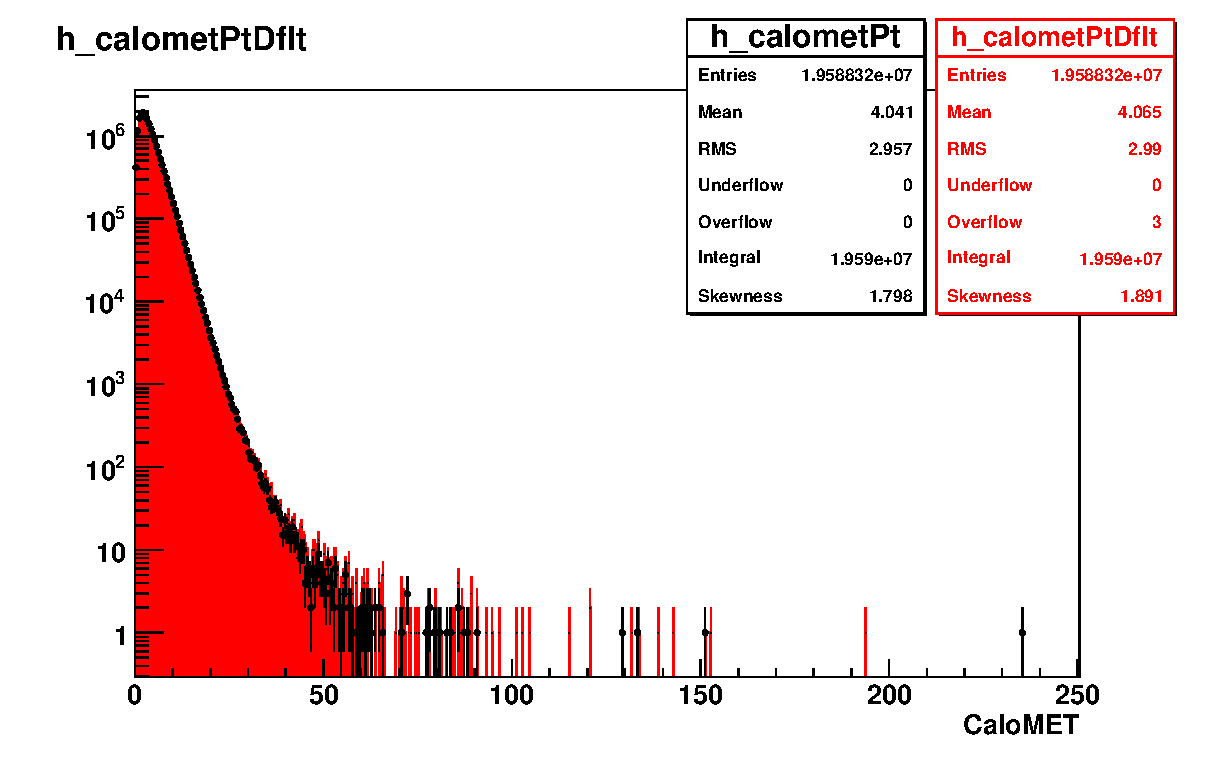
\includegraphics[width=0.7\textwidth]{fig/calomet.eps} 
 \end{tabular}
\caption{Calo$\etmiss$ distribution of 7 TeV collision data after applying the event selection described
in this section. Red filled histogram is obtained using the $\etmiss$ value coming from default CMS reconstruction 
in CMSSW\_358p3. The black dotted histogram is the $\etmiss$ after applying the full noise cleaning 
procedure described in this section.}
\label{fig:calomet}
\end{figure}